\documentclass[11pt,twocolumn]{article}

\usepackage[margin=0.78in]{geometry}
\usepackage{times}
\usepackage{latexsym}
\usepackage{microtype}
\usepackage{booktabs}
\usepackage{array}
\usepackage{tabularx}
\usepackage{graphicx}
\usepackage{url}
\usepackage[hidelinks]{hyperref}
\usepackage[round]{natbib}
\usepackage{caption}

\setlength{\columnsep}{0.24in}
\graphicspath{{../paper_assets/figures/}{paper_assets/figures/}}

\newcommand{\taskone}{Task 1}
\newcommand{\tasktwo}{Task 2}
\newcommand{\macroF}{macro-F1}

\title{Transformer Fine-Tuning for Political Question Evasion Detection in CLARITY}

\author{Project-MMD2 Team}

\date{}

\begin{document}
\maketitle

\begin{abstract}
Political interviews often contain answers that are topically related to a question while avoiding the requested commitment. We describe a transformer fine-tuning system for the SemEval 2026 CLARITY shared task on political question evasion detection. The system addresses two settings: clarity classification into \textit{Clear Reply}, \textit{Ambivalent}, and \textit{Clear Non-Reply}, and fine-grained strategy classification over nine reply and evasion strategies. We train single-task classifiers with BERT-base, RoBERTa-large, DeBERTa-v3-base, DeBERTa-v3-large, and DeBERTa-xlarge using a simple question-answer input format, and compare class-weighted training, an input wording ablation, and a shared-encoder multi-task model. On the saved runs, DeBERTa-xlarge gives the strongest \taskone{} test result with 0.632 \macroF{}, while RoBERTa-large gives the strongest \tasktwo{} majority-consensus test result with 0.342 \macroF{}. Unanimous \tasktwo{} examples are consistently easier than majority-consensus examples, indicating that annotator disagreement is a central difficulty. Overall, strong encoders provide useful baselines, but fine-grained political evasion strategy detection remains challenging under class imbalance and pragmatic ambiguity.
\end{abstract}

\section{Introduction}

Political question answering is not only a problem of topical relevance. A response can mention the same actors, policies, or events as the question while declining to answer the requested point. Speakers may answer only part of a question, shift to a broader talking point, reject a premise, cite uncertainty, or provide a direct answer inside a long digression. Detecting these phenomena matters for computational political communication because semantic similarity alone does not distinguish a clear answer from a strategic non-answer.

The CLARITY shared task studies this problem with political question-answer pairs \citep{clarity2026,qevasion_dataset}. It follows prior work on response clarity classification and evasion taxonomies, including ``I Never Said That'' \citep{ineversaidthat}. The task has two levels. \taskone{} asks whether an answer is a \textit{Clear Reply}, \textit{Ambivalent}, or \textit{Clear Non-Reply}. \tasktwo{} asks for a fine-grained strategy label, such as \textit{Explicit}, \textit{Implicit}, \textit{Dodging}, \textit{Deflection}, or \textit{Declining to answer}.

We build a reproducible Hugging Face Transformers system \citep{wolf2020transformers} for both tasks. Our goal is to establish clean baselines and error analyses rather than to introduce a complex architecture. We compare several encoder families, evaluate simple task-specific changes, and analyze how model behavior changes under label imbalance and annotator disagreement. The main contributions are:
\begin{enumerate}
    \item a complete single-task training and evaluation pipeline for both CLARITY tasks;
    \item a comparison of BERT, RoBERTa, DeBERTa-v3, and DeBERTa-xlarge encoders \citep{devlin2019bert,liu2019roberta,he2021deberta,he2021debertav3};
    \item controlled comparisons of class weighting, input wording, model scale, and shared-encoder multi-task learning;
    \item per-class, confusion, confidence, length, and annotator-disagreement analyses.
\end{enumerate}

\section{Task and Dataset}

We use the Hugging Face dataset \texttt{ailsntua/QEvasion}. The repository expects the columns \texttt{question}, \texttt{interview\_answer}, \texttt{clarity\_label}, \texttt{evasion\_label}, \texttt{annotator1}, \texttt{annotator2}, \texttt{annotator3}, and \texttt{index}. The official training split provides labels for both tasks. The official test split provides one clarity label for \taskone{} and three annotator labels for \tasktwo{}.

All runs use an 80/20 internal split of the official training data, giving 2,758 training examples and 690 development examples. The test split has 308 examples. The split is stratified where possible: single-task \taskone{} runs stratify by clarity label, single-task \tasktwo{} runs stratify by evasion label, and the multi-task run stratifies by clarity label. All saved experiments use seed 42.

Table~\ref{tab:data} summarizes the label imbalance. \taskone{} is dominated by \textit{Ambivalent}. \tasktwo{} is more imbalanced: the largest classes are \textit{Explicit}, \textit{Dodging}, and \textit{Implicit}, while \textit{Partial/half-answer}, \textit{Clarification}, and \textit{Claims ignorance} are rare. For \tasktwo{} test evaluation, 275 of 308 examples have a majority label, 125 are unanimous, and 33 have no majority.

\begin{table}[t]
\centering
\scriptsize
\begin{tabularx}{\columnwidth}{llrXX}
\toprule
Task & Split & $N$ & Majority label & Smallest label \\
\midrule
\taskone & Dev & 690 & Ambivalent 408 (59.1\%) & Clear Non-Reply 71 (10.3\%) \\
\taskone & Test & 308 & Ambivalent 206 (66.9\%) & Clear Non-Reply 23 (7.5\%) \\
\tasktwo & Dev & 690 & Explicit 211 (30.6\%) & Partial/half-answer 16 (2.3\%) \\
\tasktwo & Test maj. & 275 & Explicit 77 (28.0\%) & Partial/half-answer 3 (1.1\%) \\
\bottomrule
\end{tabularx}
\caption{Dataset split and label-imbalance summary from the saved split and prediction files, consistent with the distribution tables in \texttt{paper\_assets/tables/}. The \tasktwo{} test row uses majority-consensus labels.}
\label{tab:data}
\end{table}

\section{System Description}

\paragraph{Input format.}
The main input template concatenates the normalized question and interview answer:
\begin{quote}
\small
\texttt{Question: \{question\} Answer: \{answer\}}
\end{quote}
An input wording ablation replaces \texttt{Answer:} with \texttt{Politician's answer:}. We do not use a natural-language-inference template.

\paragraph{Single-task classifiers.}
For each task, we fine-tune \texttt{AutoModelForSequenceClassification}. \taskone{} uses a three-way classifier and \tasktwo{} uses a nine-way classifier. The implemented pipeline saves the config snapshot, split indices and IDs, label mapping, tokenizer, best model, training history, dev and test metrics, predictions, probabilities, logits, classification reports, confusion matrices, and misclassified examples.

\paragraph{Class-weighted loss.}
The baseline loss is cross-entropy. Class-weighted experiments use inverse-frequency weights computed from the internal training split. For \taskone{}, the weights are 1.093 for \textit{Clear Reply}, 0.563 for \textit{Ambivalent}, and 3.226 for \textit{Clear Non-Reply}. For \tasktwo{}, the largest weights are assigned to the rare classes \textit{Partial/half-answer}, \textit{Clarification}, \textit{Claims ignorance}, and \textit{Declining to answer}.

\paragraph{Multi-task classifier.}
The multi-task model uses a shared transformer encoder with two linear heads. One head predicts the \taskone{} clarity label and the other predicts the \tasktwo{} strategy label. The training loss is
\[
L = L_{\mathrm{task1}} + \lambda_{\mathrm{task2}} L_{\mathrm{task2}},
\]
with \(\lambda_{\mathrm{task2}}=1.0\) in the saved configuration. The best checkpoint is selected by \tasktwo{} development \macroF{}.

\paragraph{Configurations.}
Table~\ref{tab:configs} summarizes the YAML configurations used in the saved experiments. Shared training defaults include weight decay 0.01, warmup ratio 0.1, maximum gradient norm 1.0, epoch-level evaluation and checkpointing, best-checkpoint loading by validation metric, early stopping patience 2, and one saved checkpoint. DeBERTa-v3 tokenizers are loaded with \texttt{use\_fast=false} in the configs.

\begin{table*}[t]
\centering
\scriptsize
\resizebox{\textwidth}{!}{%
\begin{tabular}{llrrrrrl}
\toprule
Config family & Encoder & Max len. & Epochs & Train/Eval bs & Accum. & LR & Precision and memory settings \\
\midrule
BERT-base T1/T2 & \texttt{bert-base-uncased} & 256 & 5 & 16/32 & 1 & 2e-5 & fp32 \\
DeBERTa-v3-base T1/T2 & \texttt{microsoft/deberta-v3-base} & 256 & 6 & 8/16 & 2 & 1.5e-5 & fp16 \\
DeBERTa-v3-base weighted & \texttt{microsoft/deberta-v3-base} & 256 & 6 & 8/16 & 2 & 1.5e-5 & fp16, class weights \\
DeBERTa-v3-base alt input & \texttt{microsoft/deberta-v3-base} & 256 & 6 & 8/16 & 2 & 1.5e-5 & fp16, alternate prefix \\
RoBERTa-large T1/T2 & \texttt{roberta-large} & 256 & 5 & 2/4 & 8 & 1e-5 & fp16, grad. checkpointing \\
DeBERTa-v3-large T1/T2 & \texttt{microsoft/deberta-v3-large} & 256 & 5 & 2/4 & 8 & 1e-5 & fp16 \\
DeBERTa-xlarge T1/T2 & \texttt{microsoft/deberta-xlarge} & 192 & 4 & 1/2 & 16 & 8e-6 & fp32, grad. checkpointing \\
DeBERTa-v3-base multi-task & \texttt{microsoft/deberta-v3-base} & 256 & 6 & 8/16 & 2 & 1.5e-5 & fp16, \(\lambda_{\mathrm{task2}}=1.0\) \\
\bottomrule
\end{tabular}
}
\caption{Configuration summary for the saved runs. ``Accum.'' is gradient accumulation steps; train/eval batch sizes are per device.}
\label{tab:configs}
\end{table*}

\section{Experimental Setup}

Training uses Hugging Face \texttt{Trainer}. Models are evaluated on the internal development split after each epoch, and the best checkpoint is loaded at the end. The primary metric is \macroF{}. We also report weighted-F1 and accuracy. The analysis assets compute 95\% bootstrap confidence intervals over examples for the main \macroF{} values; these intervals do not measure training-seed variance.

\taskone{} test evaluation uses the single clarity label. \tasktwo{} test evaluation uses three annotator labels. We report majority-consensus \macroF{} on examples with at least two agreeing annotators, unanimous-only \macroF{} on examples where all three annotators agree, and any-annotator match rate over all 308 test examples. Rows without a majority are treated as unresolved annotation disagreement rather than as standard majority-label errors.

\section{Results}

\subsection{\taskone{}: Clarity Classification}

Table~\ref{tab:task1} reports \taskone{} results. DeBERTa-v3-large has the highest development \macroF{} at 0.690, while DeBERTa-xlarge has the highest test \macroF{} at 0.632 with a 95\% bootstrap interval of 0.554--0.692. Figure~\ref{fig:t1main} shows the same test comparison. The ranking suggests that the largest model helps on the held-out test set, but the differences among RoBERTa-large, DeBERTa-v3-large, and DeBERTa-v3-base are modest.

\begin{table*}[t]
\centering
\small
\begin{tabular}{lrrrr}
\toprule
System & Dev \macroF{} & Test \macroF{} & Test weighted-F1 & Test acc. \\
\midrule
BERT-base & 0.576 & 0.570 & 0.671 & 0.692 \\
DeBERTa-v3-base & 0.664 & 0.605 & 0.688 & 0.688 \\
DeBERTa-v3-base + weighted & 0.631 & 0.546 & 0.656 & 0.653 \\
DeBERTa-v3-base + alt input & 0.671 & 0.588 & 0.684 & 0.679 \\
DeBERTa-v3-base multi-task & 0.676 & 0.586 & 0.694 & 0.688 \\
RoBERTa-large & 0.677 & 0.596 & 0.671 & 0.669 \\
DeBERTa-v3-large & \textbf{0.690} & 0.595 & 0.699 & \textbf{0.698} \\
DeBERTa-xlarge & 0.687 & \textbf{0.632} & \textbf{0.701} & 0.695 \\
\bottomrule
\end{tabular}
\caption{\taskone{} development and test results. The main metric is \macroF{}.}
\label{tab:task1}
\end{table*}

\begin{figure*}[t]
\centering
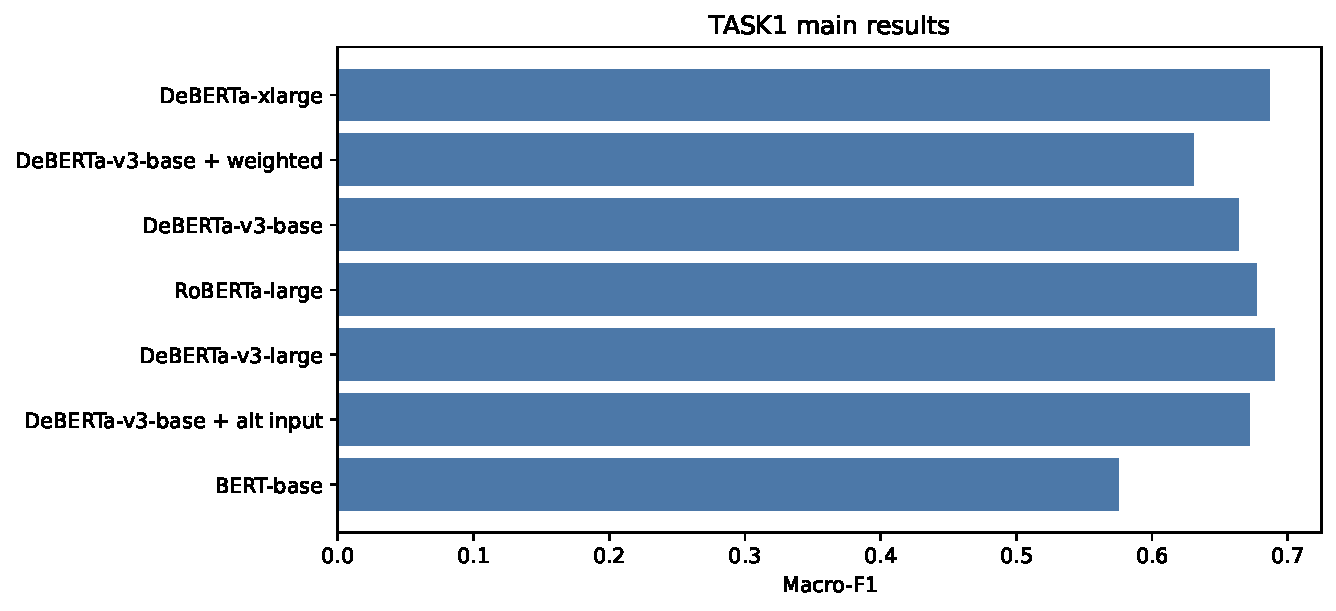
\includegraphics[width=0.92\textwidth]{main_results_task1.pdf}
\caption{\taskone{} test \macroF{} across saved systems. DeBERTa-xlarge is strongest on the test set, while class-weighted DeBERTa-v3-base is weaker than the unweighted DeBERTa-v3-base baseline.}
\label{fig:t1main}
\end{figure*}

\subsection{\tasktwo{}: Fine-Grained Strategy Classification}

Table~\ref{tab:task2} reports \tasktwo{} results. RoBERTa-large is best on both development and majority-consensus test \macroF{}, with 0.375 on development and 0.342 on test. Its test bootstrap interval is 0.239--0.402. DeBERTa-v3-large is second by majority \macroF{} and has the highest majority accuracy. Figure~\ref{fig:t2main} shows that all systems remain below 0.35 majority-consensus \macroF{} on the test set, indicating that the fine-grained strategy task is substantially harder than the coarse clarity task.

\begin{table*}[t]
\centering
\small
\begin{tabular}{lrrrr}
\toprule
System & Dev \macroF{} & Test maj. \macroF{} & Test weighted-F1 & Test maj. acc. \\
\midrule
BERT-base & 0.335 & 0.239 & 0.255 & 0.305 \\
DeBERTa-v3-base & 0.300 & 0.301 & 0.334 & 0.400 \\
DeBERTa-v3-base + weighted & 0.331 & 0.318 & 0.278 & 0.280 \\
DeBERTa-v3-base + alt input & 0.277 & 0.238 & 0.308 & 0.378 \\
DeBERTa-v3-base multi-task & 0.280 & 0.262 & 0.354 & 0.404 \\
RoBERTa-large & \textbf{0.375} & \textbf{0.342} & 0.338 & 0.385 \\
DeBERTa-v3-large & 0.368 & 0.325 & \textbf{0.380} & \textbf{0.418} \\
DeBERTa-xlarge & 0.336 & 0.267 & 0.356 & 0.400 \\
\bottomrule
\end{tabular}
\caption{\tasktwo{} development and test results. Test scores use majority-consensus labels on the 275 test examples where at least two annotators agree.}
\label{tab:task2}
\end{table*}

\begin{figure*}[t]
\centering
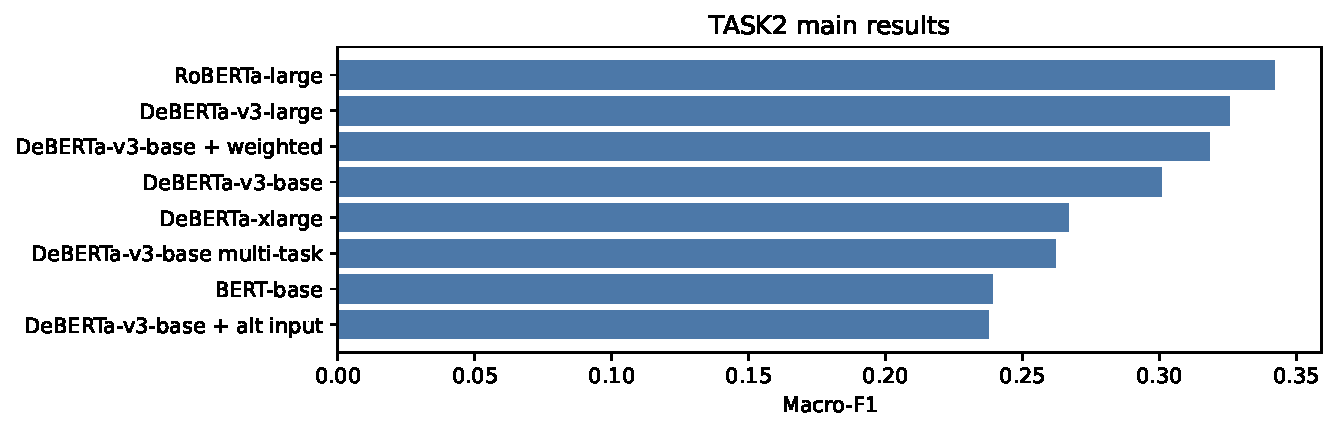
\includegraphics[width=0.92\textwidth]{main_results_task2.pdf}
\caption{\tasktwo{} majority-consensus test \macroF{} across saved systems. RoBERTa-large is the strongest saved model, followed by DeBERTa-v3-large and class-weighted DeBERTa-v3-base.}
\label{fig:t2main}
\end{figure*}

Annotator agreement changes the interpretation of \tasktwo{} results. Figure~\ref{fig:t2disagree} compares majority-consensus and unanimous-only evaluation. Unanimous-only \macroF{} is higher for every saved system. RoBERTa-large obtains 0.342 majority \macroF{} and 0.402 unanimous \macroF{}; class-weighted DeBERTa-v3-base obtains the highest unanimous-only score, 0.426, but has lower majority accuracy and any-annotator match rate. DeBERTa-v3-large has the highest any-annotator match rate at 0.542.

\begin{figure*}[t]
\centering
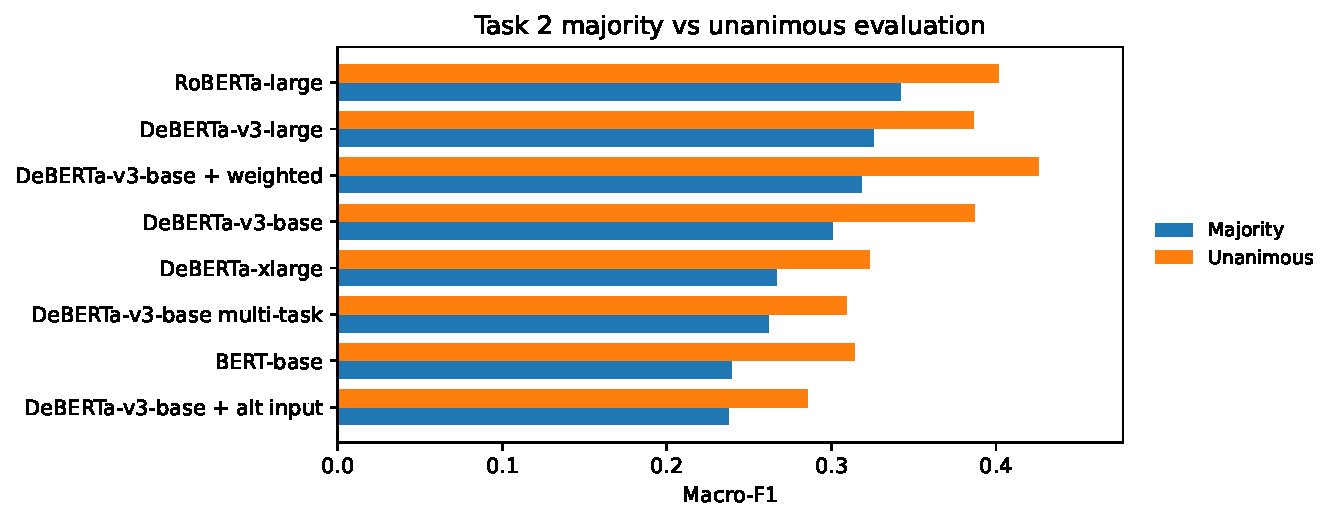
\includegraphics[width=0.92\textwidth]{task2_majority_vs_unanimous.pdf}
\caption{\tasktwo{} majority-consensus versus unanimous-only \macroF{}. Higher unanimous-only scores show that high-agreement examples are easier for the classifiers.}
\label{fig:t2disagree}
\end{figure*}

\section{Ablation and Analysis}

\paragraph{Class weighting.}
Class weighting has different effects across tasks. For \taskone{}, weighted DeBERTa-v3-base lowers test \macroF{} from 0.605 to 0.546. For \tasktwo{}, it raises DeBERTa-v3-base majority-consensus test \macroF{} from 0.301 to 0.318, but lowers majority accuracy from 0.400 to 0.280. This pattern suggests that class weighting increases attention to minority strategies but can also increase false positives.

\paragraph{Input wording.}
The alternate prefix \texttt{Politician's answer:} does not improve the saved runs. For \taskone{}, DeBERTa-v3-base drops from 0.605 to 0.588 test \macroF{}. For \tasktwo{}, it drops from 0.301 to 0.238 majority-consensus test \macroF{}. The shorter \texttt{Answer:} prefix is therefore retained.

\paragraph{Model scale.}
Increasing model size helps \taskone{} more than \tasktwo{}. DeBERTa-xlarge is best for \taskone{} test \macroF{}, but RoBERTa-large is best for \tasktwo{}. DeBERTa-v3-large is competitive on \tasktwo{} and has the highest any-annotator match rate, but the xlarge DeBERTa run does not improve the fine-grained strategy metric.

\paragraph{Multi-task learning.}
The shared-encoder model improves \taskone{} development \macroF{} over single-task DeBERTa-v3-base, 0.676 versus 0.664, but lowers \taskone{} test \macroF{} to 0.586. For \tasktwo{}, it is below the single-task DeBERTa-v3-base run on both development and majority-consensus test \macroF{}. The simple equal-weight objective is therefore not sufficient to make the two tasks help each other reliably.

\section{Error Analysis}

The best \taskone{} system, DeBERTa-xlarge, performs best on the majority class. Its per-class test F1 is 0.765 for \textit{Ambivalent}, 0.576 for \textit{Clear Reply}, and 0.553 for \textit{Clear Non-Reply}. The most common errors are \textit{Ambivalent} predicted as \textit{Clear Reply} (47 examples), \textit{Clear Reply} predicted as \textit{Ambivalent} (26 examples), and \textit{Clear Non-Reply} predicted as \textit{Ambivalent} (10 examples). Figure~\ref{fig:t1conf} shows that non-replies are often softened into the ambiguous middle category.

\begin{figure}[t]
\centering
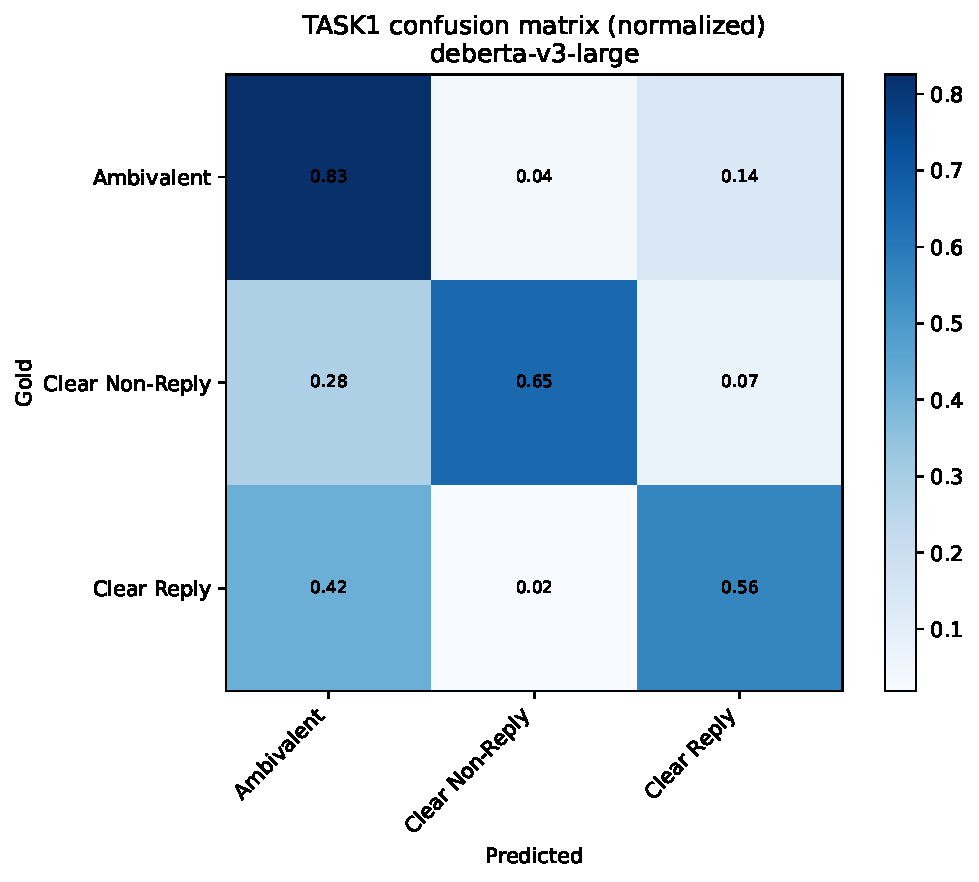
\includegraphics[width=\columnwidth]{confusion_matrix_task1_normalized.pdf}
\caption{Normalized \taskone{} confusion matrix for DeBERTa-xlarge on test. The largest off-diagonal errors involve \textit{Ambivalent} versus \textit{Clear Reply} and \textit{Clear Non-Reply} versus \textit{Ambivalent}.}
\label{fig:t1conf}
\end{figure}

For \tasktwo{}, RoBERTa-large has very uneven per-class behavior. Figure~\ref{fig:t2perclass} shows high F1 for \textit{Clarification} and \textit{Explicit}, but 0.000 F1 for \textit{Partial/half-answer}, 0.127 for \textit{Implicit}, and 0.133 for \textit{General}. The low-support classes should be interpreted cautiously, but the pattern aligns with the confusion table: \textit{Implicit} is often predicted as \textit{Explicit} or \textit{Dodging}, and \textit{General} is often predicted as \textit{Dodging} or \textit{Explicit}. Figure~\ref{fig:t2conf} visualizes these confusions.

\begin{figure}[t]
\centering
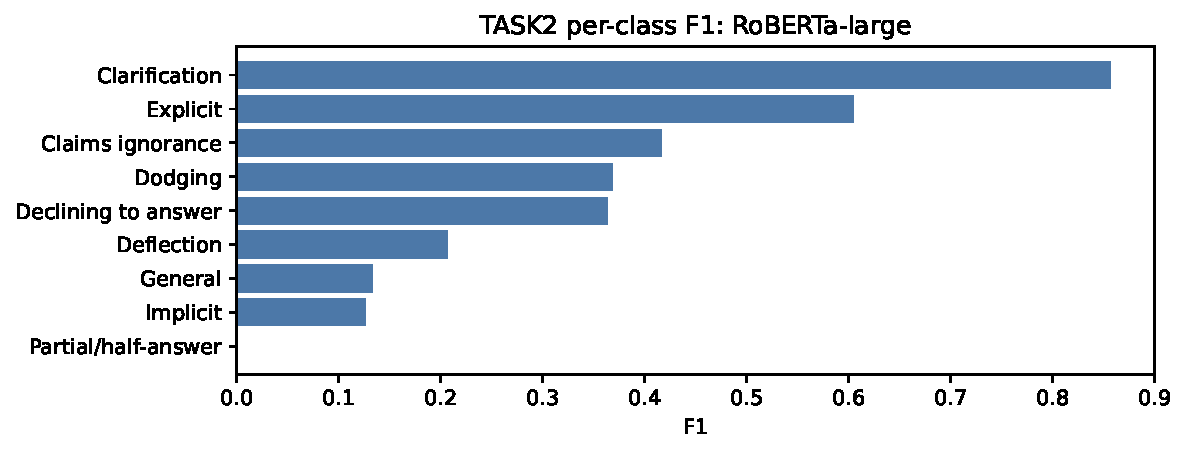
\includegraphics[width=\columnwidth]{per_class_f1_task2.pdf}
\caption{Per-class \tasktwo{} F1 for RoBERTa-large on majority-consensus test examples. Fine-grained labels differ sharply in difficulty.}
\label{fig:t2perclass}
\end{figure}

\begin{figure}[t]
\centering
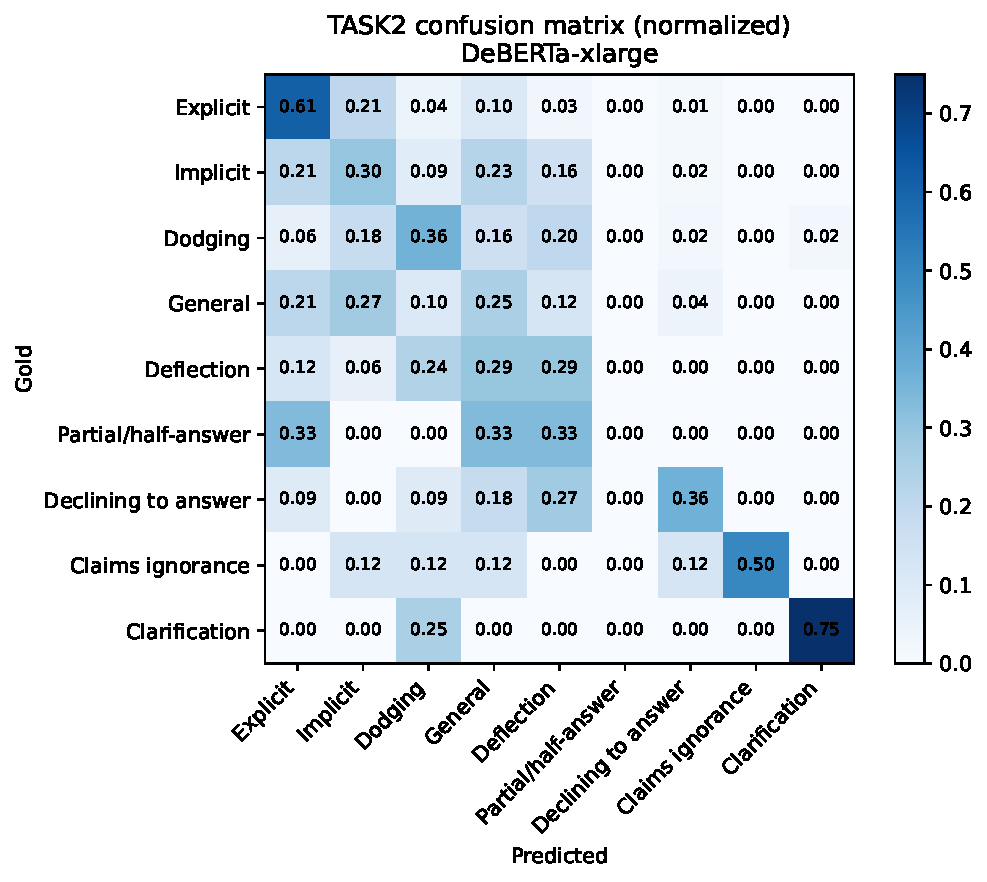
\includegraphics[width=\columnwidth]{confusion_matrix_task2_normalized.pdf}
\caption{Normalized \tasktwo{} confusion matrix for RoBERTa-large on majority-consensus test examples. Many errors concentrate around \textit{Explicit}, \textit{Dodging}, and \textit{Implicit}.}
\label{fig:t2conf}
\end{figure}

Table~\ref{tab:examples} gives representative qualitative error patterns from the saved example files. The examples show that errors often arise when an answer contains both a direct local response and broader strategic framing.

\begin{table}[t]
\centering
\small
\begin{tabularx}{\columnwidth}{p{0.14\columnwidth}p{0.30\columnwidth}X}
\toprule
Task & Gold \(\rightarrow\) prediction & Pattern \\
\midrule
\taskone & Ambivalent \(\rightarrow\) Clear Reply & A direct rejection is followed by extended framing about violence and governance. \\
\taskone & Clear Non-Reply \(\rightarrow\) Ambivalent & The answer refuses a hypothetical question but still gives related policy context. \\
\tasktwo & Implicit \(\rightarrow\) Explicit & The answer gives a plausible policy explanation without isolating the requested reason. \\
\tasktwo & General \(\rightarrow\) Dodging & The response shifts across process, regional actors, and another speaker. \\
\bottomrule
\end{tabularx}
\caption{Representative error patterns from \texttt{paper\_assets/examples/}. The table summarizes examples rather than reproducing long answers.}
\label{tab:examples}
\end{table}

\section{Additional Analysis}

\paragraph{Length and truncation.}
The saved length analysis uses approximate whitespace word counts. Test examples average 344 total words, with about 23.4\% marked as likely truncated by the analysis heuristic. In \tasktwo{}, difficult categories such as \textit{General}, \textit{Implicit}, and \textit{Partial/half-answer} have long average answer lengths in the truncation table. This supports the error analysis: long answers often mix a partial answer with background, justification, or topic shifts.

\paragraph{Confidence.}
Confidence separates correct and incorrect predictions only partially. For the best \taskone{} test system, DeBERTa-xlarge, mean maximum probability is 0.837 overall, 0.861 on correct predictions, and 0.784 on wrong predictions. For the best \tasktwo{} test system, RoBERTa-large, the corresponding values are 0.401, 0.460, and 0.364. These gaps are useful, but high-confidence wrong examples remain.

\paragraph{Annotator disagreement.}
\tasktwo{} disagreement is substantial: 33 of 308 test rows have no majority label. Majority-consensus evaluation gives a single reference label for 275 examples, while unanimous-only evaluation covers 125 high-agreement examples. The consistent increase from majority to unanimous \macroF{} in Figure~\ref{fig:t2disagree} suggests that model difficulty is partly tied to human label uncertainty.

\section{Limitations}

The saved experiments use a single seed per configuration, so model comparisons do not estimate training-seed variance. The bootstrap intervals quantify example-level uncertainty only. The dataset is imbalanced, especially for minority \tasktwo{} strategies, and many political answers are pragmatically ambiguous even for human annotators. The large-model configurations are constrained by GPU memory, using small per-device batches, gradient accumulation, and in some cases shorter maximum sequence length. The length and truncation analyses use whitespace-based approximations rather than tokenizer-specific token counts.

\section{Conclusion}

We present a reproducible transformer fine-tuning system for the CLARITY shared task on political question evasion detection. DeBERTa-xlarge is the strongest saved \taskone{} model with 0.632 test \macroF{}, while RoBERTa-large is the strongest saved \tasktwo{} model with 0.342 majority-consensus test \macroF{}. Class weighting helps the fine-grained \tasktwo{} macro metric for DeBERTa-v3-base but hurts \taskone{}, and the simple shared-encoder multi-task model does not consistently outperform single-task training. Future work should evaluate multiple seeds, stronger hierarchical models, calibrated decision rules, rationale-aware supervision, prompt-based large language model systems, and training objectives that model annotator disagreement directly.

\bibliographystyle{plainnat}
\bibliography{references}

\end{document}
